%%%%%%%%%%%%%%%%%%%%%%%%%%%%%%%%%%%%%%%%%
% Beamer Presentation
% LaTeX Template
% Version 1.0 (10/11/12)
%
% This template has been downloaded from:
% http://www.LaTeXTemplates.com
%
% License:
% CC BY-NC-SA 3.0 (http://creativecommons.org/licenses/by-nc-sa/3.0/)
%
%%%%%%%%%%%%%%%%%%%%%%%%%%%%%%%%%%%%%%%%%

%----------------------------------------------------------------------------------------
%	PACKAGES AND THEMES
%----------------------------------------------------------------------------------------

\documentclass{beamer}

\mode<presentation> {

% The Beamer class comes with a number of default slide themes
% which change the colors and layouts of slides. Below this is a list
% of all the themes, uncomment each in turn to see what they look like.

%\usetheme{default}
%\usetheme{AnnArbor}
%\usetheme{Antibes}
%\usetheme{Bergen}
%\usetheme{Berkeley}
%\usetheme{Berlin}
%\usetheme{Boadilla}
%\usetheme{CambridgeUS}
%\usetheme{Copenhagen}
%\usetheme{Darmstadt}
%\usetheme{Dresden}
%\usetheme{Frankfurt}
%\usetheme{Goettingen}
%\usetheme{Hannover}
%\usetheme{Ilmenau}
%\usetheme{JuanLesPins}
%\usetheme{Luebeck}
\usetheme{Madrid}
%\usetheme{Malmoe}
%\usetheme{Marburg}
%\usetheme{Montpellier}
%\usetheme{PaloAlto}
%\usetheme{Pittsburgh}
%\usetheme{Rochester}
%\usetheme{Singapore}
%\usetheme{Szeged}
%\usetheme{Warsaw}

% As well as themes, the Beamer class has a number of color themes
% for any slide theme. Uncomment each of these in turn to see how it
% changes the colors of your current slide theme.

%\usecolortheme{albatross}
%\usecolortheme{beaver}
%\usecolortheme{beetle}
%\usecolortheme{crane}
%\usecolortheme{dolphin}
%\usecolortheme{dove}
%\usecolortheme{fly}
%\usecolortheme{lily}
%\usecolortheme{orchid}
%\usecolortheme{rose}
%\usecolortheme{seagull}
%\usecolortheme{seahorse}
%\usecolortheme{whale}
%\usecolortheme{wolverine}

%\setbeamertemplate{footline} % To remove the footer line in all slides uncomment this line
%\setbeamertemplate{footline}[page number] % To replace the footer line in all slides with a simple slide count uncomment this line

%\setbeamertemplate{navigation symbols}{} % To remove the navigation symbols from the bottom of all slides uncomment this line
}

\usepackage{graphicx} % Allows including images
\usepackage{dirtytalk}
\usepackage{subfig}
\usepackage{booktabs} % Allows the use of \toprule, \midrule and \bottomrule in tables

%----------------------------------------------------------------------------------------
%	TITLE PAGE
%----------------------------------------------------------------------------------------

\title[ROBUST PORTFOLIO OPTIMIZATION]{ROBUST PORTFOLIO OPTIMIZATION:\\
A STUDY OF BSE30 AND BSE100} % The short title appears at the bottom of every slide, the full title is only on the title page

\author{Mohammed Bilal Girach \\ Shashank Oberoi} % Your name
\institute[]{
Department of Mathematics \\ % Your institution for the title page
\medskip
%\textit{john@smith.com} % Your email address
IIT Guwahati
}
%\date{\today} % Date, can be changed to a custom date
\date{November 15, 2018}

\begin{document}

\begin{frame}
\titlepage % Print the title page as the first slide
\end{frame}

\begin{frame}
\frametitle{Outline} % Table of contents slide, comment this block out to remove it
\tableofcontents % Throughout your presentation, if you choose to use \section{} and \subsection{} commands, these will automatically be printed on this slide as an overview of your presentation
\end{frame}

%----------------------------------------------------------------------------------------
%	PRESENTATION SLIDES
%----------------------------------------------------------------------------------------

%------------------------------------------------
\section{Motivation} % Sections can be created in order to organize your presentation into discrete blocks, all sections and subsections are automatically printed in the table of contents as an overview of the talk
%------------------------------------------------

%\subsection{Subsection Example} % A subsection can be created just before a set of slides with a common theme to further break down your presentation into chunks

\begin{frame}{Motivation}{Drawbacks of Markowitz Portfolio Optimization}
%\frametitle{Introduction}
\begin{itemize}
    \item {Can assign extreme weights to the securities.
    \begin{enumerate}
        \item{Large negative weights (practically unviable).}
        \item{Zero weights to many securities and large positive weights to small-cap stocks (with no-shortselling constraints).}\\
    \end{enumerate} 
    }
    \item {Sensitivity issue with estimates of input parameters.
    \begin{enumerate}
        \item {\say{Estimation-error maximizers} property: Overweighs securities having higher estimated mean, lower variance and negative correlation between returns.}
        \item{ Over-estimation of optimal portfolios: Estimated efficient frontier lies above the actual frontier.}
        \item{ Estimation errors in means of asset returns have a greater impact on portfolio performance in comparison to that of errors in variances/covariances of asset returns.}
    \end{enumerate}
    }
\end{itemize}
\end{frame}

%------------------------------------------------

\begin{frame}{Motivation}{Addressing the Problem}

\begin{block}{Robust Portfolio Optimization}
Class of methods proposed to enhance the robustness of Markowitz portfolios by optimizing the portfolio performance in worst-case scenarios.\\
Most of the robust models deal with optimizing a given objective function with a predefined \say{uncertainty set} for obtaining computationally tractable solutions.
\end{block}
%\textbf{Robust Portfoio Optimization}: 
%\frametitle{Bullet Points}
% \begin{itemize}
% \item Lorem ipsum dolor sit amet, consectetur adipiscing elit
% \item Aliquam blandit faucibus nisi, sit amet dapibus enim tempus eu
% \item Nulla commodo, erat quis gravida posuere, elit lacus lobortis est, quis porttitor odio mauris at libero
% \item Nam cursus est eget velit posuere pellentesque
% \item Vestibulum faucibus velit a augue condimentum quis convallis nulla gravida
% \end{itemize}
\end{frame}

%------------------------------------------------
\section{Robust Models Using Uncertainty Sets}

\begin{frame}{Robust Models Using Uncertainty Sets}{Uncertainty Sets}
\begin{itemize}
    \item Robust optimization involves defining the proper structure of uncertainty sets that will provide tractable solutions.
    \item Since the distribution of asset returns is not known with certainty, a general approach is to define some geometry around an estimate of the uncertain parameter.
    \item Empirically, the uncertain parameters are often estimated using historical returns.
    \item Even though there has been intensive study on the structure and geometry of uncertainty sets that are suitable for various optimization problems, we only cover a few types of uncertainty sets which are widely used in portfolio optimization.
\end{itemize}
\end{frame}
\begin{frame}{Robust Models Using Uncertainty Sets}{Box Uncertainty in Expected Returns (Without Short-Selling)}
A \textit{polytopic} uncertainty set which resembles a \say{box} is defined as:
\begin{equation}
\label{eqn:box}
U_{\mathbf{\delta}}(\hat{\mathbf{a}}) = \left\{ \mathbf{a} : | a_i - \hat{a}_i| \leq \delta_i, i = 1,2,3,...,N \right\},
\end{equation}
where $\mathbf{a} = (a_1, a_2, ..., a_N)$ is a vector of values of uncertain parameters of dimension $N$ and $\mathbf{\hat{a}} = (\hat{a}_1, \hat{a}_2, ... , \hat{a}_N)$ is generally the estimate for $\mathbf{a}$.
\vfill
The robust formulation of the mean-variance
model that focuses on optimizing the portfolio in the worst-case is expressed as:
\begin{equation}
\label{eq:rf}
\max_{\mathbf{x}} \left\{ \min_{\boldsymbol{\mu} \in U_{\boldsymbol{\delta}}(\boldsymbol{\hat{\mu}})} \boldsymbol{\mu}^{\top} \mathbf{x} - \lambda \mathbf{x^{\top}}\Sigma \, \mathbf{x} \right\} \text{such that } \mathbf{x^{\top}}\mathbf{1}  = 1 \text{ and } \mathbf{x} \geq 0, 
\end{equation}
where $\boldsymbol{\mu}$ represents the vector of expected returns, $\Sigma$ represents the variance-covariance matrix, $\mathbf{x}$ stands for the vector of weights for an individual asset in the optimal portfolio, $\lambda$ represents the risk-aversion of the investor and $\mathbf{1}$ represents the unity vector.
\end{frame}
\begin{frame}{Robust Models Using Uncertainty Sets}{Box Uncertainty in Expected Returns (Without Short-Selling)}

Box uncertainty in terms of expected returns can be expressed as 
\begin{equation}
U_{\boldsymbol{\delta}}(\boldsymbol{\hat{\mu}}) = \left\{ \boldsymbol{\mu}: | \mu_i - \hat{\mu_i}| \leq \delta_i, i = 1,2,3,...,N \right\},    
\end{equation}
where $N$ represents the number of stocks and $\delta_i$ represents the value which determines the confidence interval region for individual assets. On incorporating the box uncertainty set, the formulation in (\ref{eq:rf}) 
transforms to a maximization problem
\begin{equation}
\label{eqn:trans_eqn_box}
\max_\mathbf{x} \quad \boldsymbol{\hat{\mu}}^{\top} \, \mathbf{x}-  \lambda \mathbf{x^{\top}}\Sigma \, \mathbf{x} - \boldsymbol{\delta}^{\top}|\mathbf{x}| \quad \text{such that } \mathbf{x^{\top}}\mathbf{1}  = 1 \text{ and } \mathbf{x} \geq 0,  
\end{equation}
\vfill
While dealing with the box uncertainty, it is assumed that the returns follow normal distribution.  We define $\delta_i$ for $100(1 - \alpha)\%$ confidence level as follows: $$ \delta_i = \sigma_{i} \, z_\frac{\alpha}{2} \, N^{-\frac{1}{2}}$$
\end{frame}
\begin{frame}{Robust Models Using Uncertainty Sets}{Ellipsoidal Uncertainty in Expected Returns (Without Short-Selling)}
On the same lines, in this context, we define Ellipsoidal uncertainty sets in terms of expected returns as follows:
\begin{equation}
U_{\delta}(\boldsymbol{\hat{\mu}}) = \left\{ \boldsymbol{\mu} : (\boldsymbol{\mu} - \boldsymbol{\hat{\mu}})^{\top} \, \Sigma^{-1}_{\boldsymbol{\mu}} \, (\boldsymbol{\mu} - \boldsymbol{\hat{\mu}}) \leq \delta^2 \right\},
\end{equation}

where $\Sigma_\mu$ is the covariance matrix of the estimated errors in expected returns. Again, by this model, the optimization problem (\ref{eq:rf}) transforms to 
\begin{equation}
\max_{\mathbf{x}} \left\{ \boldsymbol{\hat{\mu}}^{\top} \mathbf{x} - \lambda \mathbf{x}^{\top} \, \Sigma \, \mathbf{x} - \delta \sqrt{\mathbf{x}^{\top} \, \Sigma_{\boldsymbol{\mu}} \, \mathbf{x}} \right\} \text{such that } \mathbf{x^{\top}} \mathbf{1}  = 1 \text{ and } \mathbf{x} \geq 0.
\end{equation}
For the same reason, if the uncertainty set follows ellipsoid model, the underlying distribution is assumed to be tracing a $\chi_N^2$ distribution. Accordingly, for $100(1-\alpha)\%$ confidence level, $\delta$ can be computed as: $$\delta^2=\chi_{N}^2(\alpha)$$
where $\chi_{N}^2(\alpha)$ is the inverse of a chi square distribution with $N$ degrees of freedom.
\end{frame}
\begin{frame}{Robust Models Using Uncertainty Sets}{Separable Uncertainty Set (Without Short-Selling)}

In this type, we obtain the bounds for both the covariance matrix and the expected returns.
$U_{\boldsymbol{\mu}}= \{\boldsymbol{\mu}: \underline{\boldsymbol{\mu}} \leq \boldsymbol{\mu} \leq \overline{\boldsymbol{\mu}} \}$, where $\underline{\boldsymbol{\mu}}$ and $\overline{\boldsymbol{\mu}}$ represent lower and upper bounds on mean return vector $\boldsymbol{\mu}$ respectively .
Lower bound $\underline{\Sigma}_{ij}$ and upper bound $\overline{\Sigma}_{ij}$ can be specified for each entry $\Sigma_{ij}$ of the covariance matrix.

From this we transform the problem (\ref{eq:rf}) to the following:
\begin{equation}
\begin{split}
& \max_{\mathbf{x}} \left\{ \underline{\boldsymbol{\mu}}^{\top} \mathbf{x} - \lambda \mathbf{x^{\top}} \, \overline{\Sigma} \, \mathbf{x} \right\} \text{such that } \mathbf{x^{\top}} \mathbf{1}  = 1 \text{ and } \mathbf{x} \geq 0.  \\
\end{split}
\end{equation}

\vfill
We obtain the bounds of both mean vectors and the covariance matrix by using non-parametric bootstrap algorithm.


\end{frame}

% \begin{frame}{Tune $\delta$'s and obtain bounds}
%     \begin{itemize}
%         \item While dealing with the box uncertainty, it is assumed that the returns follow normal distribution as it eases the task of computing the desired confidence intervals for each individual asset. We define $\delta_i$ for $100(1 - \alpha)\%$ confidence level as follows: $$ \delta_i = \sigma_{i} \, z_\frac{\alpha}{2} \, n^{-\frac{1}{2}}$$
%         \item For the same reason, if the uncertainty set follows ellipsoid model, the underlying distribution is assumed to be tracing a $\chi^2$ distribution with the number of assets being the degrees of freedom (df). Accordingly, for $100(1-\alpha)\%$ confidence level, $\delta$ is defined in the following manner $$\delta^2=\chi_{N}^2(\alpha)$$
%         where $\chi_{N}^2(\alpha)$ is the inverse of a chi square distribution with $N$ degrees of freedom.
%     \end{itemize}
% \end{frame}
\section{Computational Results}

\begin{frame}{Computational Results}{Implementation Details}
\begin{itemize}
    \item{Analysis performed under two scenarios:
    \begin{enumerate}
        \item{Number of stocks $N=31$}
        \item{Number of stocks $N=98$}
    \end{enumerate}
    }
    \item{For each scenario, following data used:
    \begin{enumerate}
        \item{Log-returns based on daily Adjusted Close Price of stocks comprising BSE30 for Scenario 1 and BSE100 for Scenario 2 (Yahoo Finance).}
        \item{Simulated Data with $\#$samples for returns same as in market data.}
        \item{Simulated Data with $\#$samples$=1000$}
    \end{enumerate}
    }
    \item{Sharpe Ratio used as performance measure for comparing robust models with Markowitz Model (Mark) with annualized risk-free rate assumed equal to $6\%$.}
    \item{Portfolio optimization within ideal range of risk-aversion ($\lambda \in [2,4]$). }
    \item{Uncertainty sets constructed with $95\%$ confidence level. }
\end{itemize}
\end{frame}

\begin{frame}{Computational Results}{Performance with $N=31$ assets}
\begin{figure}[!h]
    %\centering
    %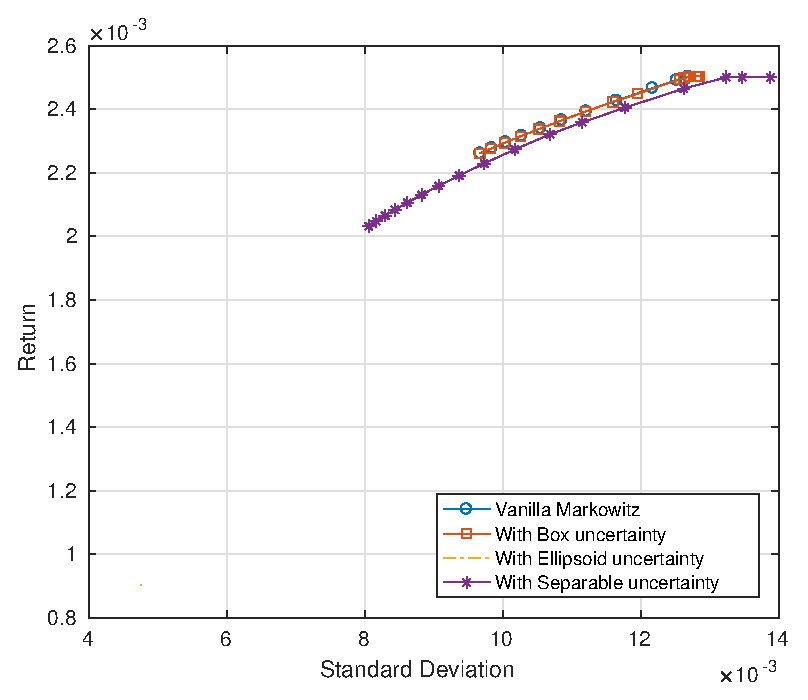
\includegraphics{bse30_simulated/ef_ideal_range_1000_sim.eps}
    %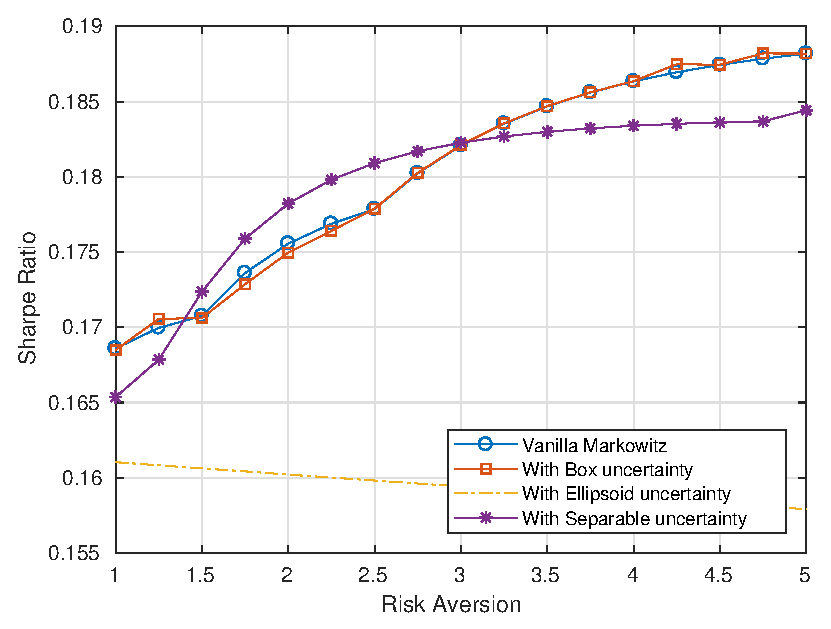
\includegraphics{bse30_simulated/sr_ideal_range_1000_sim.eps}
    
    
    \subfloat{\includegraphics[height=3.825cm,width=0.3\textwidth]{bse30_market/ef_ideal_range.eps}} \hspace{5mm}
   \subfloat{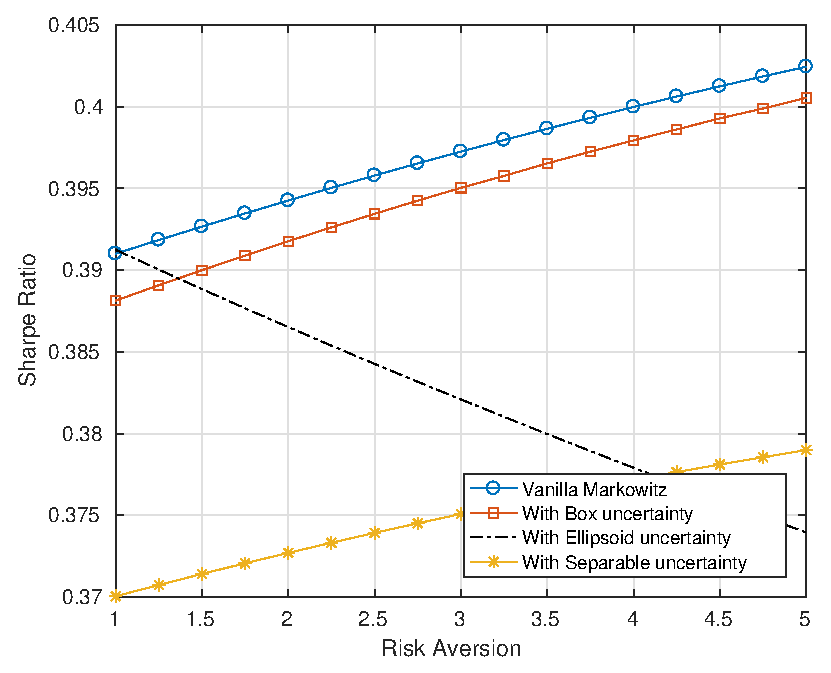
\includegraphics[height=3.7cm,width=0.32\textwidth]{bse30_market/sr_ideal_range.eps}}\\
   \caption{\centering{Efficient Frontier plot and Sharpe ratio plot for different portfolio optimization models in case of Market Data (31 assets)}}
   \label{fig:1}
\end{figure}
\end{frame}

\begin{frame}{Computational Results}{Performance with $N=31$ assets}
\begin{table}[!h]
    \centering
    \small
    \captionsetup{justification=centering}
  %\begin{tabular}{|c|c|c|c|c|c|c|c|c|c|c|c|c|}
  \begin{tabular}{||c|c|c|c|c||}
  \hline
  
%   $\lambda$ & $\sigma_{Mark}$ & $\mu_{Box}$ & $\sigma_{Box}$ & $\mu_{Ellip}$ & $\sigma_{Ellip}$ & $\mu_{Sep}$ & $\sigma_{Sep}$ & $S_{Mark}$ & $S_{Box}$ & $S_{Ellip}$ & $S_{Sep}$ \\
  
  $\lambda$ & $SR_{Mark}$ & $SR_{Box}$ & $SR_{Ellip}$ & $SR_{Sep}$ \\
  
  \hline
 2 & 0.181 & 0.181 & 0.193 & 0.186 \\
 2.5 & 0.181 & 0.181 & 0.192 & 0.193 \\
 3 & 0.186 & 0.191 & 0.192 & 0.202 \\
 3.5 & 0.194 & 0.195 & 0.191 & 0.209 \\
 4 & 0.201 & 0.202 & 0.19 & 0.213 \\
  \hline
  Avg & 0.189 & 0.19 & 0.192 & 0.2 \\
  \hline

\end{tabular}
    \caption{\centering{Comparison of different portfolio optimization models in case of Market Data (31 assets)}}
    \label{tab:1}
\end{table}
\begin{block}{Common observation inferred from three cases}
Sep and Ellip model perform superior or equivalent in comparison to Markowitz model in the ideal range of risk-aversion.
\end{block}
\end{frame}   



\begin{frame}{Computational Results}{Performance with $N=98$ assets}

\begin{figure}[!h]
    %\centering
    %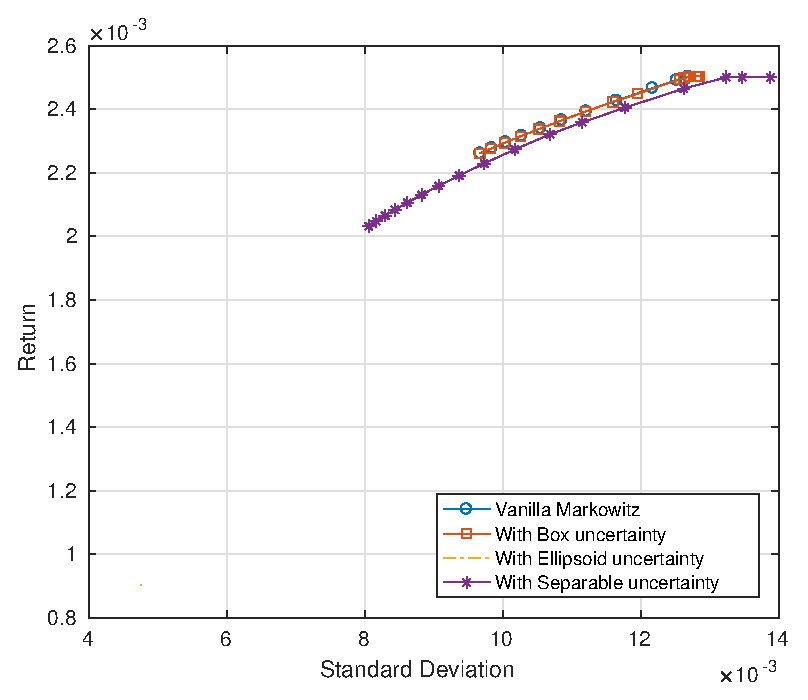
\includegraphics{bse30_simulated/ef_ideal_range_1000_sim.eps}
    %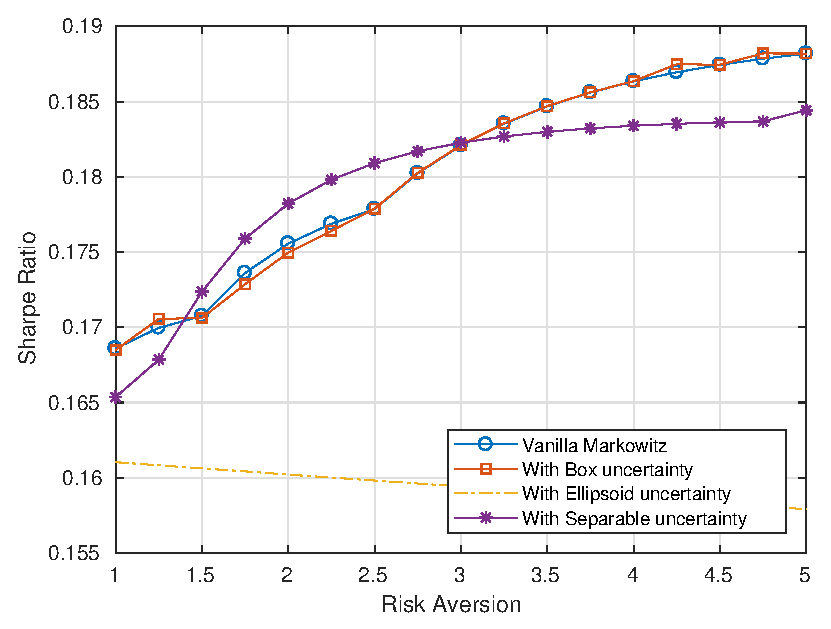
\includegraphics{bse30_simulated/sr_ideal_range_1000_sim.eps}
    
    
    \subfloat{\includegraphics[height=3.825cm,width=0.3\textwidth]{bse100_market/ef_ideal_range.eps}} \hspace{5mm}
   \subfloat{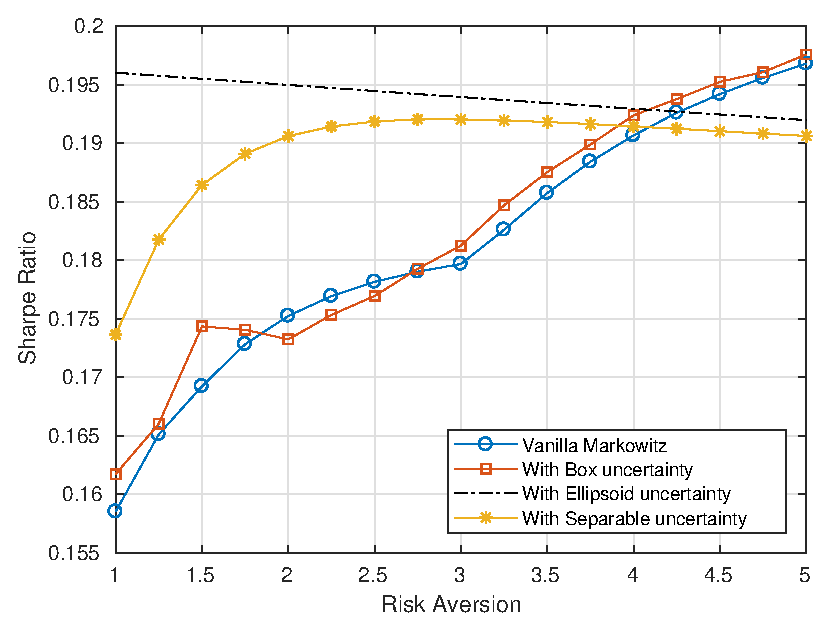
\includegraphics[height=3.7cm,width=0.32\textwidth]{bse100_market/sr_ideal_range.eps}}\\
   \caption{\centering{Efficient Frontier plot and Sharpe ratio plot for different portfolio optimization models in case of Market Data (98 assets)}}
   \label{fig:2}
\end{figure}
    
\end{frame}

\begin{frame}{Computational Results}{Performance with $N=98$ assets}

\begin{table}[!h]
    \centering
    \small
    \captionsetup{justification=centering}
   %\begin{tabular}{|c|c|c|c|c|c|c|c|c|c|c|c|c|}
   \begin{tabular}{||c|c|c|c|c||}
   \hline
  
%   $\lambda$ & $\sigma_{Mark}$ & $\mu_{Box}$ & $\sigma_{Box}$ & $\mu_{Ellip}$ & $\sigma_{Ellip}$ & $\mu_{Sep}$ & $\sigma_{Sep}$ & $S_{Mark}$ & $S_{Box}$ & $S_{Ellip}$ & $S_{Sep}$ \\
  
  $\lambda$ & $SR_{Mark}$ & $SR_{Box}$ & $SR_{Ellip}$ & $SR_{Sep}$ \\
  
  \hline
2 & 0.175 & 0.173 & 0.195 & 0.193 \\
2.5 & 0.178 & 0.177 & 0.194 & 0.193 \\
3 & 0.18 & 0.181 & 0.194 & 0.193 \\
3.5 & 0.186 & 0.188 & 0.193 & 0.192 \\
4 & 0.191 & 0.192 & 0.193 & 0.192 \\
  \hline
  Avg & 0.182 & 0.182 & 0.194 & 0.192 \\
  \hline

\end{tabular}
    \caption{Comparison of different portfolio optimization models in case of Market Data (98 assets)}
    \label{tab:2}
\end{table} 

\begin{block}{Common observation inferred from three cases}
Sep and Ellip model outperform the Markowitz model in the ideal range of risk-aversion.
\end{block}

\end{frame}

\section{Conclusions and Comments}

\begin{frame}{Conclusions and Comments}{From the Standpoint of Number of Stocks}
\begin{table}[!h]
    \centering
    \small
    \captionsetup{justification=centering}
   %\begin{tabular}{||p{6cm}|p{3cm}|p{3cm}||}
   \begin{tabular}{||c|c|c||}
   \hline
  & \#stocks = 31 & \#stocks = 98 \\
  \hline
 \#generated\textunderscore simulations = 1000  & 0.2    &0.244\\
 \#generated\textunderscore simulations = $\zeta$ & 0.218  & 0.233 \\
 Market data & 0.2 & 0.194 \\
 \hline
\end{tabular}
    \caption{\centering{The maximum average Sharpe ratio compared by varying the number of stocks in different kinds of scenarios.}}
    \label{tab:no_stocks}
\end{table}
\begin{block}{Qualitative argument for this observation}
More the number of stocks, more is the diversification of the portfolio. This is the principle behind this type of observation. However, in market data, the Sharpe ratio in case of more number of stocks is less than that of the case with smaller number of stocks. We believe that this kind of behaviour is due to relatively low amount of data available for higher number of stocks.
\end{block}
\vfill
\end{frame}

\begin{frame}{Conclusions and Comments}{From the Standpoint of Number of Samples Generated}

\begin{table}[!h]
    \centering
    \small
    \captionsetup{justification=centering}
   %\begin{tabular}{||p{4cm}|p{4cm}|p{4cm}||}
   \begin{tabular}{||c|c|c||}
   \hline
  & \#samples = 1000 & \#samples = $\zeta$ \\
  \hline
  \#stocks = 31  & 0.2    &0.218\\
 \#stocks = 98 &   0.244  & 0.233 \\
 \hline
\end{tabular}
    \caption{The maximum average Sharpe ratio compared by varying the number of stocks in different kinds of scenarios.}
    \label{tab:no_samples}
\end{table}
\begin{block}{Qualitative argument for this observation}
We explain this type of behaviour as follows: In the available real market data, the number of instances available for larger number of stocks is relatively low. So, when  more number of samples were generated, we observe higher Sharpe ratios when compared to $\zeta$ number of simulations. We are yet to explore the reason behind such type of behaviour when smaller number of stocks are considered.
\end{block}
\vfill
\end{frame}

\begin{frame}{Conclusions and Comments}{From the Standpoint of Type of the Data}
\begin{table}[!h]
    \centering
    \small
    \captionsetup{justification=centering}
   %\begin{tabular}{||p{4cm}|p{4cm}|p{4cm}||}
   \begin{tabular}{||c|c|c||}
   \hline
  & Simulated data & Real Market data \\
  \hline
  \#stocks = 31  & 0.218    &0.2\\
 \#stocks = 98 &   0.244  & 0.194  \\
 \hline
\end{tabular}
    \caption{The maximum average Sharpe ratio compared by varying the type of the data in different kinds of scenarios.}
    \label{tab:data_type}
\end{table}
\begin{block}{Qualitative argument for this observation}
Here the behaviour is straight forward. In both the cases, the performance in the case of simulated data is better than the real market data. This is clear from the fact that the real market data are difficult to model and hardly may follow any distribution, whereas the simulated data simply follows multivariate normal distribution with mean and covariances as the true values obtained from the data.
\end{block}
\vfill
\end{frame}



\section{Take-Aways}

\begin{frame}{Take-Aways}

\begin{itemize}
    \item {In contrast to the results reported by Scherer (used simulated data), we observe that robust optimization with ellipsoidal uncertainty set performs superior or equivalent as compared to Markowitz model in the case of simulated data as well as market data. This could be attributed to incorporation of no short-selling constraints in the optimization problem.  }
    \item {Better performance of robust formulation having separable uncertainty set in comparison to Markowitz model is in line with the previous study on the same robust model by T{\"u}t{\"u}nc{\"u} and Koenig.}
\end{itemize}
    
\end{frame}

\section{Future Directions}

\begin{frame}{Future Directions}
\begin{itemize}
    \item Extending robust optimization techniques to a framework involving multi-period investment.
    \item Incorporating coherent measures of risk like AVaR in the robust models
\end{itemize}
\end{frame}




%------------------------------------------------



%------------------------------------------------
%\section{Second Section}
%------------------------------------------------



%------------------------------------------------



%------------------------------------------------





% \begin{frame}[fragile] % Need to use the fragile option when verbatim is used in the slide
% \frametitle{Citation}
% An example of the \verb|\cite| command to cite within the presentation:\\~

% This statement requires citation \cite{p1}.
% \end{frame}

%------------------------------------------------
\section{References}

\begin{frame}
\frametitle{References}
\footnotesize{
\begin{thebibliography}{99} % Beamer does not support BibTeX so references must be inserted manually as below
% \bibitem[Smith, 2012]{p1} John Smith (2012)
% \newblock Title of the publication
% \newblock \emph{Journal Name} 12(3), 45 -- 678.
\bibitem{mark1} H. M. Markowitz. Portfolio selection. The journal of finance, 7(1):77–91,
1952.
\bibitem{michaud} R. O. Michaud. The markowitz optimization enigma: Is ’optimized’ optimal? Financial Analysts Journal, 45(1):31–42, 1989.
\bibitem{broadie} M. Broadie. Computing efficient frontiers using estimated parameters. Annals of Operations Research, 45(1):21–58, Dec 1993.
\bibitem{black} F. Black and R. Litterman. Global portfolio optimization. Financial Analysts Journal, 48(5):28–43, 1992.
\bibitem{tut} R. H. T{\"u}t{\"u}nc{\"u} and M. Koenig. Robust asset allocation. Annals of Operations Research, 132(1-4):157–187, 2004.
\bibitem{scherer} B. Scherer. Can robust portfolio optimisation help to build better portfolios? Journal of Asset Management, 7(6):374–387, Mar 2007.
\bibitem{fabozzi} F. J. Fabozzi, P. N. Kolm, D. Pachamanova, and S. M. Focardi. Robust Portfolio Optimization and Management. Wiley, 2007.
\end{thebibliography}
}
\end{frame}

%------------------------------------------------

\begin{frame}
\Huge{\centerline{The End}}
\end{frame}

%----------------------------------------------------------------------------------------

\end{document}